\documentclass[12pt]{article}
\usepackage[margin=1in,letterpaper]{geometry}
\usepackage{graphicx}
\usepackage{amssymb}
\usepackage{amsmath}
\usepackage{palatino}
\usepackage{mathpazo}
\usepackage{color}
\usepackage{hyperref}
\usepackage{multirow}
\usepackage{braket}
\usepackage{relsize}
\usepackage{color, colortbl}
\usepackage{booktabs}
\usepackage[dvipsnames]{xcolor}
\definecolor{darkblue}{RGB}{46,48,147}
\hypersetup{colorlinks=true,
            linkcolor=darkblue,
            urlcolor=darkblue,
            citecolor=darkblue}
\definecolor{Gray}{gray}{0.9}
\definecolor{LightCyan}{rgb}{0.88,1,1}
\definecolor{LightRed}{rgb}{1,0.92,0.92}
\newcommand{\solColor}{blue}
\newcommand{\sol}{\color{\solColor}}
\newcommand*\publistbasestyle{phys}
\usepackage[style=publist,
biblabel=brackets,
sorting=dt,
plauthorhandling=highlight,
nameorder=given-family,
]{biblatex}
\DeclareSourcemap{
 \maps[datatype=bibtex,overwrite=true]{
  \map{
    \step[fieldsource=Collaboration, final=true]
    \step[fieldset=usera, origfieldval, final=true]
  }
 }
}
\renewbibmacro*{author}{
  \iffieldundef{usera}{
    \printnames{author}
  }{
    \printfield{usera} Collaboration
  }
}
\addbibresource{syllabus.bib}

\begin{document}

\begin{center}
	\textbf{University of California San Diego\\
		Department of Physics\\
		Physics 139/239, Winter 2023\\
		Machine Learning in Physics (4 units)}
\end{center}

\begin{figure}[h!]
	\centering
	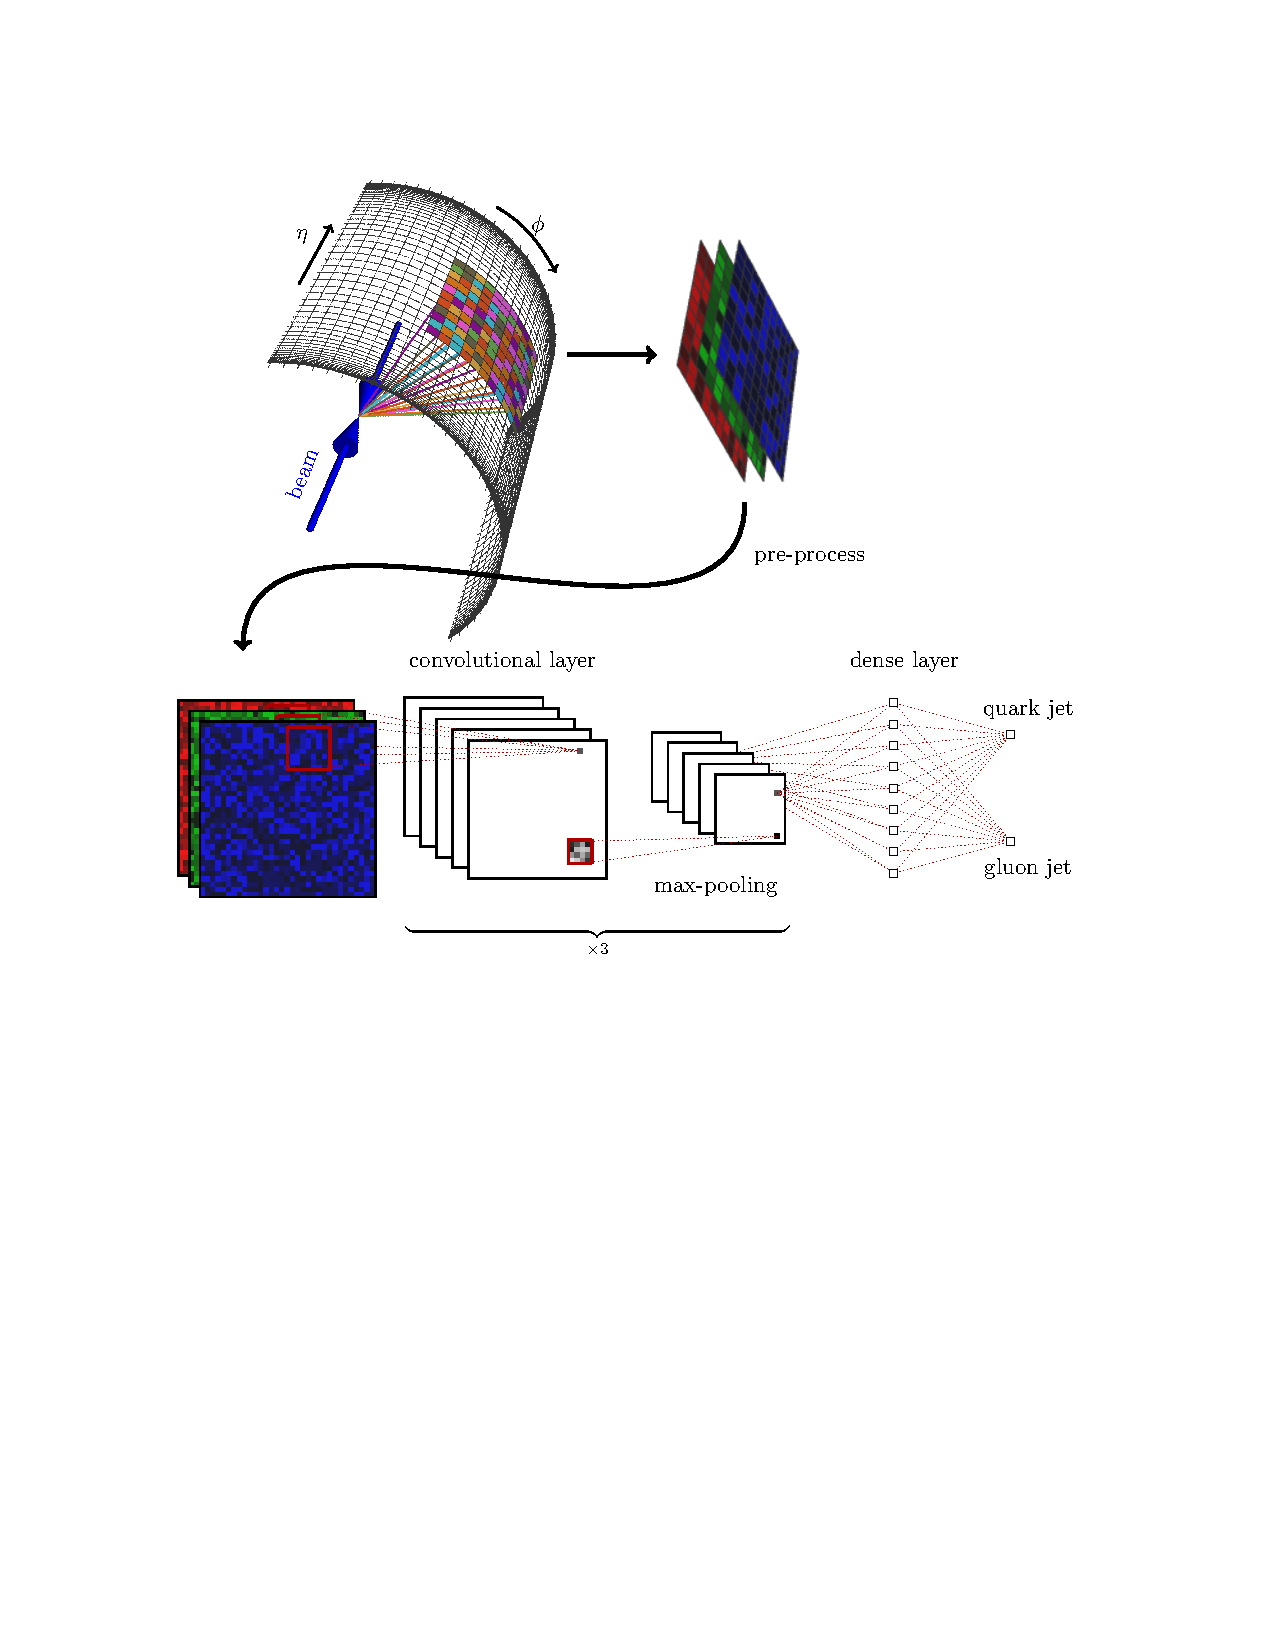
\includegraphics[width=0.7\textwidth]{quark_gluon.pdf}
\end{figure}

\noindent\textbf{Instructor}: Javier Duarte, \href{mailto:jduarte@ucsd.edu}{jduarte@ucsd.edu}, OH TBD, Zoom TBD
%\noindent \textbf{Teaching assistants}:\\
%\hspace*{1cm}Yiwen Huang, \href{mailto:yih003@ucsd.edu}{yih003@ucsd.edu}, OH Th 11:00--11:50am, Zoom \href{https://ucsd.zoom.us/j/93414311658}{934 1431 1658}\\
%\hspace*{1cm}Ruoyu Yin, \href{mailto:yruoyu@ucsd.edu}{yruoyu@ucsd.edu}, OH Tu \& Th 9:30--10:20pm, Zoom \href{https://ucsd.zoom.us/j/94960939850}{949 6093 9850}\\

%\noindent\textbf{Course webpage, Zoom link to lectures}:\\
%\hspace*{1cm}Login through \href{http://canvas.ucsd.edu}{http://canvas.ucsd.edu}; Zoom links can be accessed through Canvas.\\
%\hspace*{1cm}All assignments will be due through Canvas or Gradescope (accessed through Canvas).\\
%\hspace*{1cm}All content that you will need will be available on Canvas.\\

\begin{center}
	\rule{\textwidth}{0.5pt}
\end{center}

\noindent\textbf{Course information}: This course is an upper-division undergraduate course and introductory graduate course on machine learning in physics.
No previous machine learning knowledge is necessary.
However, some basic knowledge of calculus, linear algebra, statistics, and Python programming may be expected/useful.

The course structure will consist of weekly lectures on conceptual topics, e.g. statistics, linear algebra, scientific data set exploration, feature engineering, (stochastic) gradient descent, neural networks, and unsupervised learning.
Students will learn key concepts in data science and machine learning, including selecting and preprocessing data, designing machine learning models, evaluating model performance, and relating model inputs and outputs to the underlying physics concepts.
We will apply these methods to the domains of collider physics, neutrino physics, astronomy, and potentially others.
There will be 4--6 homework assignments.
There will also be a final project in which students will work in groups to reproduce the results of a ML in physics research article.
A midterm assignment to propose the project will also be required.

\begin{center}
	\rule{\textwidth}{0.5pt}
\end{center}

\noindent\textbf{Course Schedule}:
\begin{center}
	\begin{tabular}{|l|c|l|m{50mm}|}
		\hline
		Lecture    & TuTh         & 12:30p--1:50p & SOLIS 109, Zoom TBD    \\\hline
		Final exam & Tu 3/21/2023 & 11:30a-2:29p  & Location TBD, Zoom TBD \\\hline
	\end{tabular}
\end{center}

\noindent\textbf{First lecture}: Tu 1/10/2023

\begin{center}
	\rule{\textwidth}{0.5pt}
\end{center}

\noindent\textbf{Textbook}: There is no required textbook for this course.
At the end of the syllabus, we list a bibliography of (mostly free) textbooks and online resources we will draw from.

\begin{center}
	\rule{\textwidth}{0.5pt}
\end{center}

\noindent\textbf{Student learning outcomes}: Upon successful completion of Physics 139/239, students will be able to:
\begin{itemize}
	\item Find, explore, select, and preprocess scientific data
	\item Choose and design machine learning models
	\item Evaluate model performance and compare to standard benchmarks
	\item Debug machine learning workflows
	\item Relate model inputs and outputs to underlying physics concepts
	\item Collaborate with peers to tackle complex, realistic problems
	\item Present findings
\end{itemize}

\begin{center}
	\rule{\textwidth}{0.5pt}
\end{center}

\noindent\textbf{Grading policy}: Your final course grade will be determined according to the following:
\begin{itemize}
	\item $\sim$50\% Homework.
	\item $\sim$10\% Participation in class/via Slack.
	\item $\sim$20\% Midterm: Written proposal for group project.
	\item $\sim$20\% Final: Written group project summary, presentation, self-evaluation, and code.
\end{itemize}
with the exact breakdown to be determined.

\begin{center}
	\rule{\textwidth}{0.5pt}
\end{center}

\noindent\textbf{Drop policy}: The lowest homework score is dropped automatically.
This drop policy is designed to account for any and all illnesses, family, medical, mental, or other emergencies.

If you have an extended emergency (e.g., a long hospital stay) that hinders your ability to turn complete assignments beyond the emergency policy allowance, contact the professor directly as soon as the situation arises.

\begin{center}
	\rule{\textwidth}{0.5pt}
\end{center}

\noindent\textbf{Discussion board}: We will use Slack.

\begin{center}
	\rule{\textwidth}{0.5pt}
\end{center}

\noindent\textbf{Homework}: Each homework will consist of a set of programming challenges.
The assignments will be submitted as Jupyter notebooks or GitHub repositories.

There will be a first deadline to submit a ``draft'' version of the homework, which will be graded based on effort.

There will be a second deadline to submit a ``final'' version of the homework, which will be graded based on effort and correctness.

\begin{center}
	\rule{\textwidth}{0.5pt}
\end{center}

\noindent\textbf{Midterm and Final Project}:
For the final project, students will work in groups to reproduce the results of a ML in physics research article.
Students will also be required to submit a written proposal for the project around Week 6--7.
This is to ensure the project is feasible and to receiver feedback form instructors.

\begin{center}
	\rule{\textwidth}{0.5pt}
\end{center}

\noindent\textbf{Attendance (lectures)}: You are not required to come to the lectures, but your attendance is strongly recommended.
The lecture hours will be split into conceptual and practical parts, with interactive problem-solving and pair programming throughout.
These sessions will be recorded.

\begin{center}
	\rule{\textwidth}{0.5pt}
\end{center}

\noindent\textbf{Academic integrity}: Please read the College Policies section of the \href{http://senate.ucsd.edu/Operating-Procedures/Senate-Manual/Appendices/2}{UCSD’s Policy on Integrity of Scholarship}.
These rules will be enforced.
Cheating includes, but is not limited to: submitting another person's work as your own, copying from any person/source, and using any unauthorized materials or aids during exams.

For homework assignments, copying from an online solution, a peer's solution, a Chegg solution, or shared work (on Discord, for example) is considered cheating.
Collaboration is encouraged, but by the time you start writing your own solution to turn in, you should not be looking at any other source.
You should know the rough outline of the solution well enough that you do not need to reference something line-by-line.
Plagiarizing a solution but changing variable names is considered cheating.
Soliciting help online via Chegg, Quora, etc. is considered cheating.
If suspected, you might be asked to rework similar problems in a Zoom one-on-one meeting with the instructor and/or TA.

Any questions on what constitutes an academic integrity violation should be addressed to the instructor; any violation of academic integrity will result in immediate reporting to the UCSD Office of Academic Integrity, and can result in an automatic ``F'' for the course at the discretion of the instructor.

\begin{center}
	\rule{\textwidth}{0.5pt}
\end{center}

\noindent\textbf{Counseling and Psychological Services (CAPS):} The mission of CAPS is to promote the personal, social, and emotional growth of students.
Many services are available to UCSD students including individual, couples, and family counseling, groups, workshops, and forums, consultations and outreach, psychiatry, and peer education.
To make an appointment, call (858) 534-755.
For more information, visit \href{https://wellness.ucsd.edu/caps/}{https://wellness.ucsd.edu/caps/}.

\begin{center}
	\rule{\textwidth}{0.5pt}
\end{center}

\noindent\textbf{\emph{Preliminary Course Schedule}} ({\color{Orange} Subject to change}):\\

\textbf{Week 1}

\emph{Conceptual}: Introduction to ML, bias/variance trade-off, perceptron

\emph{Practical}: Python/Jupyter, NumPy, Git, good ML practices (e.g., training/validation/testing)

\emph{Domain}: Classifying (low-dimensional) collider events

\textbf{Week 2}

\emph{Conceptual}: Support vector machines, decision trees

\emph{Practical}: Scikit-learn, XGBoost

\emph{Domain}: Classifying (high-dimensional) collider events

\emph{Logistical}: Homework 1 due

\textbf{Week 3}

\emph{Conceptual}: Deep neural network, gradient descent, backpropagation, training issues

\emph{Practical}: Keras

\emph{Domain}: Classifying (high-dimensional) collider events

\textbf{Week 4}

\emph{Conceptual}: Convolutional neural network, image-like data

\emph{Practical}: Keras

\emph{Domain}: Classifying neutrino events and/or astronomical data (images)

\emph{Logistical}: Homework 2 due

\textbf{Week 5}

\emph{Conceptual}: Recurrent neural network, time-series data

\emph{Practical}: Docker, Kubernetes

\emph{Domain}: Identifying radio signals (time series)

\textbf{Week 6}

\emph{Conceptual}: Graph neural networks, relational inductive bias, permutation invariance and equivariance

\emph{Domain}: $N$-body simulations, springs

\emph{Logistical}: Homework 3 due

\textbf{Week 7}

\emph{Conceptual}: Unsupervised learning, clustering, autoencoders

\emph{Domain}: Finding anomalies in LHC/LIGO data

\emph{Logistical}: Project proposal due

\textbf{Week 8}

\emph{Conceptual}: \textbf{Guest Lecture}: Physics-informed neural networks

\emph{Logistical}: Homework 4 due

\textbf{Week 9}

\emph{Conceptual}: \textbf{Guest Lecture}: Equivariant neural networks

\emph{Logistical}: No homework due: work on final project

\textbf{Week 10}

\emph{Conceptual}: \textbf{Guest Lecture}: Generative models

\emph{Logistical}: No homework due: work on final project

\textbf{Finals Week}

\emph{Logistical}: Final project due

\begin{center}
	\rule{\textwidth}{0.5pt}
\end{center}

\noindent\textbf{\emph{Course Bibliography}}:\\

\textbf{Textbooks:}

\newrefsection
\nocite{Mehta:2019,Abu-Mostafa:2012,Erdman:2021,Zeljko:2014,Chollet:2021,Calafiura:2022}
\printbibliography[heading=none]

\textbf{Videos:}

\newrefsection
\nocite{3blue1brown_neuralnetwork,3blue1brown_gradientdescent}
\printbibliography[heading=none]

\textbf{Reviews:}

\newrefsection
\nocite{Carleo:2019ptp}
\printbibliography[heading=none]

\textbf{Articles:} {\color{Orange} To be updated}

\newrefsection
\nocite{deOliveira:2015xxd,Aurisano:2016jvx,Komiske:2016rsd,Khan:2018opv,Zhou:2019,Moreno:2019neq,Ormiston:2020ele,Moreno:2021fvp}
\printbibliography[heading=none]

\textbf{Datasets:} {\color{Orange} To be updated}

\newrefsection
\nocite{hbb_dataset}
\printbibliography[heading=none]

\end{document}
